\documentclass[11pt]{article}

\usepackage{a4wide}
\usepackage{mathptm}
\usepackage{xspace}
\usepackage{amsmath}
\usepackage{graphicx}
\usepackage{algorithm}
\usepackage{algpseudocode}
\usepackage{tikz}
\usepackage{tkz-graph}
\usetikzlibrary{shapes.misc, positioning}
\usepackage{listings}
\usepackage{color}

\definecolor{dkgreen}{rgb}{0,0.6,0}
\definecolor{gray}{rgb}{0.5,0.5,0.5}
\definecolor{mauve}{rgb}{0.58,0,0.82}

\lstset{frame=tb,
  language=Java,
  aboveskip=3mm,
  belowskip=3mm,
  showstringspaces=false,
  columns=flexible,
  basicstyle={\small\ttfamily},
  numbers=left,
  numberstyle=\tiny\color{gray},
  keywordstyle=\color{blue},
  commentstyle=\color{dkgreen},
  stringstyle=\color{mauve},
  breaklines=true,
  breakatwhitespace=true,
  tabsize=3
}
\begin{document}

\title{Apache Spark Software Technology Evaluation Project}

\author{Jose Juan Pena Gomez and Enrique Vilchez Campillejo}

\maketitle

\begin{abstract}

The software technology which will be discussed in this report is \textbf{Apache Spark}, an unified tool for analysing and processing data. In addition, \textbf{PySpark} is going to be used to write the code in \textbf{iPython Notebook}.

The purpose of this report is to check the different ways of processing big data using \textbf{Distributed Machine Learning} techniques, working with clusters, to see which way of \textbf{clustering} is more efficient.

The dataset taken for this project contains taxi travels with information about source location, target location, amount of passengers and taxi fare. This \textbf{large dataset} is a proficient approach to work with Spark in big data computing purposes.

There will be three Distributed Machine Learning models presented, in two approaches, one way for \textbf{Native Clustering}, which means one core acting as a cluster and the other approach is \textbf{Local Clustering} which means as many clusters as cores the processor has.

The models used are \textbf{Linear Regression}, \textbf{Decision Tree} and \textbf{Random Forest} generating several results. Basically, the results acknowledge the efficiency to work with Local Clustering rather than working with Native Clustering. 

Another improvement would be to work with \textbf{Remote Clustering} in a network with several machines, but it wasn't possible to implement it in the end. Remote clustering is more efficient because of the quantity of cores used to parallelize the tasks.

  
\end{abstract}

%\input{commands}

\section{Introduction}
\label{sec:introduction}


The main purpose of the project is to use a unified analytics engine (Apache Spark) to compare how clustering works with machine learning and how the technology works itself. As we worked before in projects of Machine Learning, we think it would be interesting to work with distributed machine-learning framework.


Approximately in 2008, the basis for creating this technology appeared, Hive and HBase, which are two tools of the Hadoop ecosystem.  
Spark was founded at UC Berkeley in 2009, it was created practically from a Google paper and since then it evolved, going through the mapreduce processes.



\noindent
\begin{figure}[H]
	\centering
	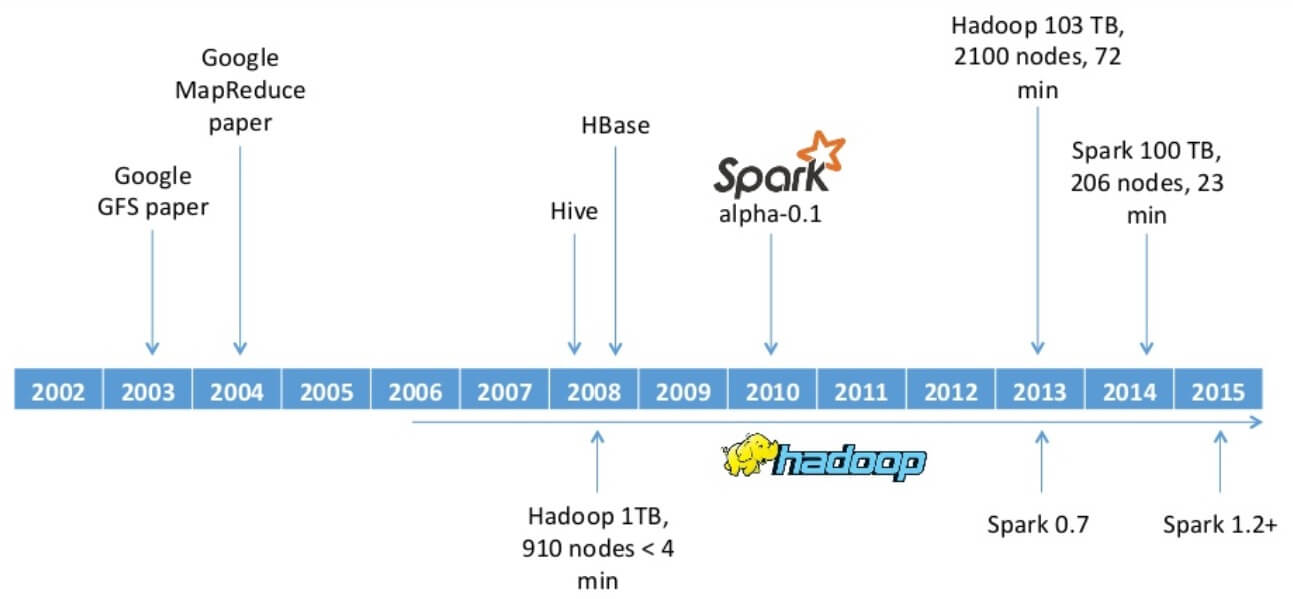
\includegraphics[scale=0.3]{figs/TimelineSpark.jpg}
	\caption{Apache Spark Development Timeline}
	\label{fig:timeline}
\end{figure}

Comparing this technology with others, for example with sklearn, the most well-known library for machine learning porposes, we are satisfied with our results. The sklearn library is not even able to load big datasets, but Apache Spark is. In addition, we are satisfied with the clustering management which is approximately 60 \% faster than without clustering management. \\*

\noindent

This rest of this report is organised as follows:

\begin{itemize}


\item Section~\ref*{sec:background} gives an overview of the key concepts and the architecture.

\item Section~\ref*{sec:prototype} gives a view of the prototype and its implementation

\item Section~\ref*{sec:experiments} gives an explanation of the test-bed environment used and the results of the experiments

\item Section~\ref*{sec:conclusion} gives a conclusion about the main concepts that is observed from this technology.

\end{itemize}
\noindent

\section{The Software Technology}
\label{sec:background}


Apache Spark is an open-source distributed general-purpose cluster-computing framework. Spark provides an interface for programming entire clusters with implicit data parallelism and fault tolerance. Originally developed at the University of California, Berkeley's AMPLab, the Spark codebase was later donated to the Apache Software Foundation, which has maintained it since. It is based on a data computing and analytics system based on Hadoop Map Reduce.

The official web defines Apache Spark as an unified analytics engine for large-scale data processing.\cite{sparkWebsite} \\*

Apache Spark has as its architectural foundation the resilient distributed dataset (RDD), a read-only multiset of data items distributed over a cluster of machines, that is maintained in a fault-tolerant way.\cite{brown:zaharia2010spark} The Dataframe API was released as an abstraction on top of the RDD, followed by the Dataset API. In Spark 1.x, the RDD was the primary application programming interface (API), but as of Spark 2.x use of the Dataset API is encouraged \cite{brown:eadline2015hadoop} even though the RDD API is not deprecated The RDD technology still underlies the Dataset API.\\*

It works in memory, which results in a much faster processing speed, it allows you to work on disk with large amount of data. In this way if for example we have a very large file or a quantity of information that does not fit in memory, the tool allows to store part in disk, which makes lose speed. This means that we have to try to find the balance between what is stored in memory and what is stored in disk, to have a good speed and so that the cost is not too high, as the memory is always much more expensive than the disk.\\*

Spark and its RDDs were developed in 2012 in response to limitations in the MapReduce cluster computing paradigm, which forces a particular linear dataflow structure on distributed programs: MapReduce programs read input data from disk, map a function across the data, reduce the results of the map, and store reduction results on disk. Spark's RDDs function as a working set for distributed programs that offers a (deliberately) restricted form of distributed shared memory.\cite{zaharia2012resilient} \\*

Spark facilitates the implementation of both iterative algorithms, which visit their data set multiple times in a loop, and interactive/exploratory data analysis, i.e., the repeated database-style querying of data. The latency of such applications may be reduced by several orders of magnitude compared to Apache Hadoop MapReduce implementation Among the class of iterative algorithms are the training algorithms for machine learning systems, which formed the initial impetus for developing Apache Spark. \\*

Apache Spark requires a cluster manager and a distributed storage system. For cluster management, Spark supports standalone (native Spark cluster, where you can launch a cluster either manually or use the launch scripts provided by the install package. It is also possible to run these daemons on a single machine for testing), Hadoop YARN, Apache Mesos or Kubernetes. For distributed storage, Spark can interface with a wide variety, including Alluxio, Hadoop Distributed File System (HDFS), MapR File System (MapR-FS), Cassandra, OpenStack Swift, Amazon S3, Kudu, Lustre file system, or a custom solution can be implemented. Spark also supports a pseudo-distributed local mode, usually used only for development or testing purposes, where distributed storage is not required and the local file system can be used instead; in such a scenario, Spark is run on a single machine with one executor per CPU core.\cite{wang2014characterization} \\*

The friendly APIs ,which Apache Spark provides, natively supports Java, Scala, R, and Python, giving you a variety of languages for building your applications. These APIs make it easy for developers, because they hide the complexity of distributed processing behind simple, high-level operators that dramatically lowers the amount of code required.\\*

It allows real time processing, with a module called Spark Streaming, which combined with Spark SQL will allow us to process the data in real time. As we are injecting the data we can transform them and turn them to a final result.
Resilient Distributed Dataset (RDD), it uses the lazy evaluation, which means that all the transformations that we are carrying out on the RDD, are not resolved, but are stored in a directed acyclic graph (DAG), and when we execute an action, that is to say, when the tool does not have more option than to execute all the transformations, it will be when they are executed. This is a double-edged sword, as it has an advantage and a disadvantage. The advantage is that you gain speed by not making transformations continuously, but only when necessary. The disadvantage is that if some transformation raises some kind of exception, it will not be detected until the action is executed, so it is more difficult to debug or program.

\subsection{Spark Architecture}

The main components that make up the framework are the following ones:

\begin{description}

	\item[Spark Core]: It is the base or set of libraries where the rest of modules are supported, is the core of the framework.It is also shelter to API that contains the backbone of Spark that is RDDs (resilient distributed datasets). The basic functionality of Spark is present in Spark Core like:
	\begin{enumerate}
		\item Memory management
		\item Fault recovery
		\item Interaction with the storage system.
		\item It is in charge of essential I/O functionalities like:
		\begin{itemize}
			\item Programming and observing the role of Spark cluster
			\item Task dispatching
			\item Fault recovery
			\item It overcomes the snag of MapReduce by using in-memory computation.\\*
		\end{itemize}
	\end{enumerate}

	

	
	
	\item[Spark SQL]: It is the module for the processing of structured and semi-structured data. With this module we will be able to transform and perform operations on RDD or dataframes. It is designed exclusively for data processing.\\*
	
	
	\item[Spark Streaming]: It is the one that allows the ingestion of data in real time. If we have a source, for example Kafka or Twitter, with this module we can ingest data from that source and dump them to a destination. Between the ingestion of data and its subsequent dump, we can have a series of transformations.\\*
	
	
	\item[Spark MLLib]: It is a very complete library that contains numerous Machine Learning algorithms, both clustering, classification, regression, and so on. It allows us, in a friendly way, to use Machine Learning algorithms.
	
	
	\item[Spark Graph]: Allows the processing of graphs (DAG). It does not allow to paint graphs, but it allows to create operations with graphs, with their nodes and edges, and to go making operations.\\*
	
\end{description}


\begin{figure}[h]
	\centering
	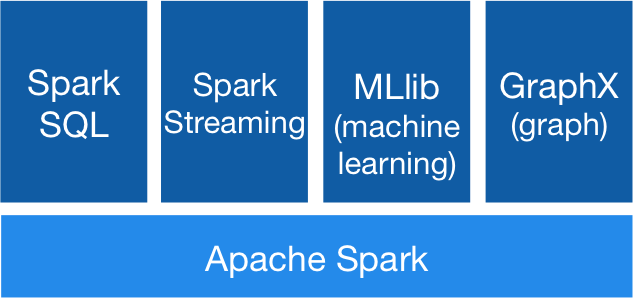
\includegraphics[scale=0.65]{figs/spark-components.png}
	\caption{Components of Apache Spark}
	\label{fig:components-spark}
\end{figure}

\subsection{MLlib}

MLIB is part of Spark APIs and is interoperable with Python NumPy as well as the R libraries. Implemented with Spark it is possible to use any type of data from any source or from the Hadoop platform such as HDFS, HBase, related database data sources or local data sources such as text documents.\\*

Spark excels in iterative calculation processes allowing the processes written in the MLlib libraries to be executed quickly allowing their use and above all at an industrial level.\\*

MLlib provides many types of algorithms, as well as numerous useful functions. ML includes classification algorithms, regression, decision trees, recommendation algorithms, grouping. Among the most used utilities can include the characteristics of transformations, standardization and normalization, statistical functions and linear algebra.\\*

\subsection{Clustering}



Apache Spark can be configured to run on distributed mode on the cluster as a master node or slave node. Its master/slave architecture is composed by many main daemons and a cluster manager. T schedules and divides resource in the host machine which forms the cluster. 
\begin{itemize}

	\item Master Daemon — (Master/Driver Process)
	\item Worker Daemon –(Slave Process)
	\item Cluster Manager. Schedules and divides resources in the host machine which forms the cluster
\end{itemize}

As we can see in the figure~\ref{fig:clusters-spark} .
\begin{figure}[h]
	\centering
	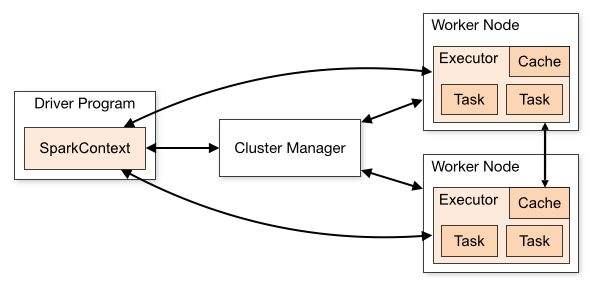
\includegraphics[scale=0.5]{figs/cluster-overview.png}
	\caption{Cluster management of Apache Spark}
	\label{fig:clusters-spark}
\end{figure}



\section{Demonstrator Prototype}
\label{sec:prototype}

About 5 pages that gives:

\begin{enumerate}
  
\item High-level view of the demonstrator and its purpose.

\item Details of how the demonstrator has been implemented.

\item May involve presentation of code snippets.

\end{enumerate}

The example below shows how you may include code. There are similar
styles for many other langages - in case you do not use Java in your
project. You can wrap the listing into a figure in case you need to
refer to it. How to create a figure was shown in Section~\ref{sec:background}.
  
\lstinputlisting[language=java]{code/BoksVolum.java}


\section{Test-bed Environment and Experimental Results}
\label{sec:experiments}

About 3 pages that:

\begin{description}

\item[Describes] the software used to establish the test-bed and for implementing the demonstrator prototype.

\item[Explains] what experiments have been done and the results.

\end{description}

For some reports you may have to include a table with experimental
results are other kinds of tables that for instance compares
technologies. Table~\ref{tab:results} gives an example of how to create a table.

\begin{table}
\centering
\begin{tabular}{llrrrrrr}
  Config & Property & States & Edges & Peak & E-Time & C-Time & T-Time
  \\ \hline \hline
22-2 & A   &    7,944  &   22,419  &  6.6  \%  &  7 ms & 42.9\% &  485.7\% \\   
22-2 & A   &    7,944  &   22,419  &  6.6  \%  &  7 ms & 42.9\% &  471.4\% \\   
30-2 & B   &   14,672  &   41,611  &  4.9  \%  & 14 ms & 42.9\% &  464.3\% \\   
30-2 & C   &   14,672  &   41,611  &  4.9  \%  & 15 ms & 40.0\% &  420.0\% \\ \hline
10-3 & D   &   24,052  &   98,671  & 19.8  \%  & 35 ms & 31.4\% &  285.7\% \\   
10-3 & E   &   24,052  &   98,671  & 19.8  \%  & 35 ms & 34.3\% &  308.6\% \\
\hline \hline
\end{tabular}
\caption{Selected experimental results on the communication protocol example.}
\label{tab:results}
\end{table}

--------------------------------------------------------------------------------------------------------------------
\subsection{Jupyter Notebooks}

The software we used to experiment with the data was Jupyter Notebook to write python code and PySpark to run that python code into spark.
Jupyter Notebook (formerly IPython Notebook) is an open-source web application that lets you create and share documents containing live code, equations, visualizations, and narrative text.\\*

Also, it is a widely used application in the field of Data Science to create and share documents including data cleansing and transformation, numerical simulation, statistical modeling, data visualization, automatic learning and much more.\\*
It allows you to edit and run notebook documents through any web browser of your choice, and it can run on a local desktop that does not require Internet access, or it can be installed on a remote server and accessed through the Internet. We can also run Jupyter Notebook without any installation.

\subsection{PySpark}
PySpark is a python API for spark released by the Apache Spark community to support python with Spark. Using PySpark, one can easily integrate and work with RDD in python programming language too. 

Numerous features make PySpark such an amazing framework when it comes to working with huge datasets. Whether it is to perform computations on large data sets or to just analyze them, Data engineers are turning to this tool. Following are some of the said features.\\*

\noindent
The following features are the key features of PySpark:

\begin{description}
	\item [Real-time computations]: Because of the in-memory processing in PySpark framework, it shows low latency.
	\item [Polyglot]: PySpark framework is compatible with various languages like Scala, Java, Python, and R, which makes it one of the most preferable frameworks for processing huge datasets.
	\item [Caching and disk persistence]: PySpark framework provides powerful caching and very good disk persistence.
	\item [Fast processing]: PySpark framework is way faster than other traditional frameworks for big data processing.
	\item [Works well with RDD]: Python programming language is dynamically typed which helps when working with RDD.
\end{description}

\noindent
\subsection{About the dataset Taxi Problem} \cite{taxiDataset}

The goal of this dataset is predicting the fare amount (inclusive of tolls) for a taxi ride in New York City given the pickup and dropoff locations. While you can get a basic estimate based on just the distance between the two points, this will result in an RMSE of $5-$8, depending on the model used. Our challenge is to do it using distributed Machine Learning techniques.\\*

We also choose this dataset because contains 6 Gb of data, so we think that is a proper amount of data for test our results.

\subsection{Experiments }

We have done six experiments (Each experiment it’s a model testing), to try Linear regression, Decision tree regression and Random forest regression in Native Clustering and the rest to try Linear regression, Decision tree regression and Random forest regression in Local Cluster mode.\\*

\begin{table}[h]
	\centering
	\begin{tabular}{llrrrrrr}
		Mode & Machine Learning Model & Time-1 & RMSE-1 & Time-2 & RMSE-2 & Time-3 & RMSE-3
		\\ \hline \hline
		Native Cluster  & Linear Regression   &    4:04 min  &   20.7  &  11:47 min & 20.7 & 8:17 min & 20.7 \\   
		Native Cluster  & Decision Tree   &    8:37 min  &   23.96  &  20:22 min  &  23.96  & 20:05 min &  23.96\\   
		Native Cluster  & Random Forest   &   11:50 min &   23.96  &  35:37 min  & 24.82  & 35:53 min & 24.82 \\  \hline
		Local Cluster   & Linear Regression   &   2:33 min &   20.7  &  7:40 min  & 20.7 & 7:36 min  & 20.7   \\ 
		Local Cluster   & Decision Tree   &   5:30 min &   16.49  & 11:35 min & 24.03 & 13:05 min & 24.03  \\   
		Local Cluster   & Random Forest   &   8:44 min &   23.96  & 18:30 min & 23.96 & \textbf{26:28 min} & \textbf{6.86}  \\
		\hline \hline
	\end{tabular}
	\caption{Selected experimental results on the training models.}
	\label{tab:results}
\end{table}

We have two important approaches, one is that Linear Regression is the fastest model, and Random Forest is the worst (What it isn’t so important for our main purpose), and the other one is that clearly, with local clustering the machine invest much less time than with Native Spark training the same models respectively.
Also, it’s better to use Clustering with several machines, but we couldn’t really experiment with that.


\section{Conclusions}
\label{sec:conclusion}

Concludes on the project, including the technology, its maturity,
learning curve, and quality of the documentation.

The references used throughput the report should constitute a well
chosen set of references, suitable for someone interesting in learning
about the technology.


\bibliographystyle{plain}
\bibliography{report.bib}{}

\end{document}
